\subsection{Atollic TrueSTUDIO}

\begin{figure}[ht]
	\centering
	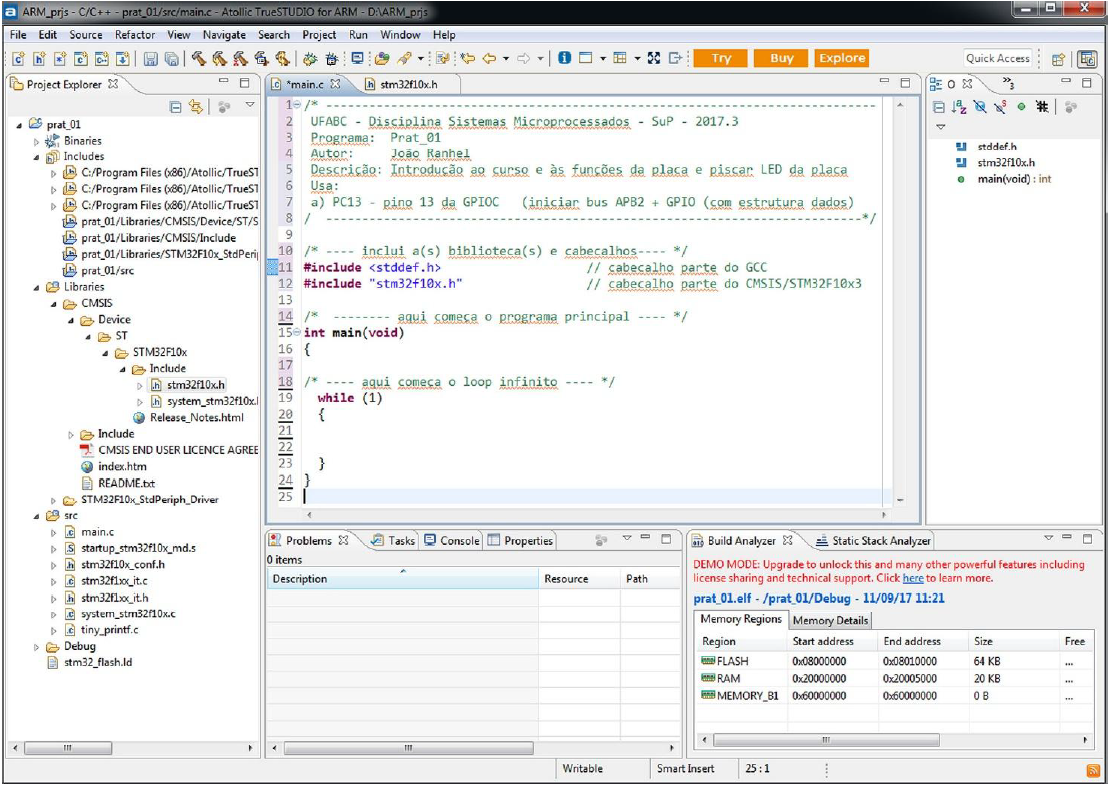
\includegraphics[width=0.8\textwidth]{figures/atollic}
	\caption{Interface Atollic \cite{apostila_microprossados}}
\end{figure}

A IDE a ser usada para programar um STM32 seria o TrueSTUDIO, distribuído pela
Atollic, que foi adquirida pela ST-Microelectronics em 2017. Trata-se de um
software livre para programar em C/C++, criado com base na plataforma Eclipse,
e que possui todas as funções esperadas para o trabalho com o STM32, tais como
edição, compilação e debugging. Uma de seus principais vantagens é não haver
limites para tamanho de projeto, o que o torna ideal para trabalhos
profissionais. O TrueSTUDIO deixou de receber atualizações em 2017,
depois da aquisição pela ST-Microelectronics.\cite{apostila_microprossados}



\subsection{Arduino IDE}

Devido a complicações nas configurações de múltiplas saídas de PWM com o
TrueSTUDIO, optou-se por usar Arduino como alternativa. Um obstáculo a essa
alternativa é que o Arduino não é compatível com STM32 nativamente,
porém o projeto Arduino\_STM32 \cite{arduino_stm32}, por Roger Clark.
O projeto contem os arquivos em C para usar o hardware do STM32 com Arduino IDE
do STM32 no Arduino. No momento de escrita deste trabalho, o projeto era
compatível apenas com a versão 1.8 da IDE do Arduino.
A IDE também é compatível com o ESP32,  usando a biblioteca arduino-esp32 \cite{arduino_esp32}, 
disponibilizada pela fabricante do microcontrolador.

Porém como o STM32 por padrão necessita do gravador ST-link, e para grava-lo usando micro-USB-B
Para habilitar esse uso, é necessário existe um projeto que modifica o software interno do STM32 para esse fim, 
\cite{stm32duino_bootloader}, porém esse processo pode impedir que o SMT32 possa ser usado  com o TrueSTUDIO e ST-link.
Embora o processo possa ser reversível, a flexibilidade do STM32 dificulta uma pesquisa em encontrar
a biblioteca ou integração apropriada para o fim desejado.

% https://docs.espressif.com/projects/esp-idf/en/v5.0/esp32s3/hw-reference/chip-series-comparison.html
% https://www.espressif.com/en/media_overview/news/20160907-esp32briefing#:~:text=Sep%207%2C%202016-,Espressif%20announces%20the%20launch%20of%20ESP32%20Cloud%20on%20Chip%20and,MCU%20at%20Shanghai%20Parkyard%20Hotel.

\begin{figure}[ht]
	\centering
	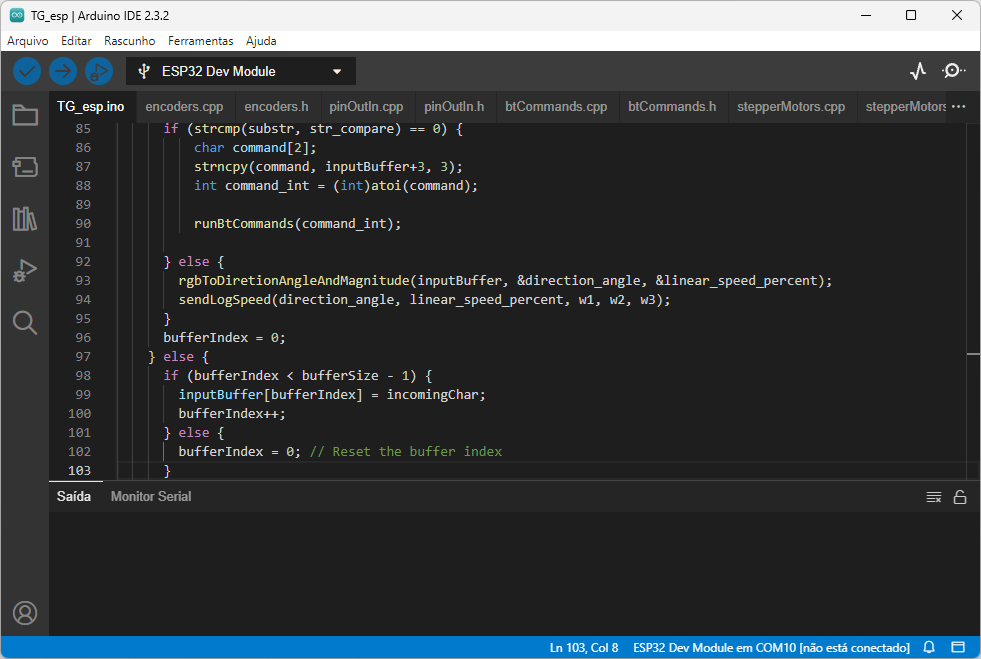
\includegraphics[width=1\textwidth]{figures/arduino}
	\caption{Interface Arduino}
\end{figure}



